\chapter{Реализация системы обработки данных} \label{chapt3}

Программная реализация алгоритмов мюонного скважинного плотномера выполнена с использованием 
программного пакета LabVIEW, библиотеки, написанной на языке C++ и алгоритмах, основанных на 
градиентном спуске, реализованных на матричном языке octave. 
На (рис. \ref{img:operator}) представлен интерфейс оператора по вводу и обработке тарировочных данных. 
Тарировочные данные вводятся таблично. После введения данных проводится контроль их корректности.  
При запуске начальной аппроксимации (кнопка «Аппроксимировать») отображается аппроксимационная 
кривая с наименьшей погрешностью, график погрешности в зависимости от текущего параметра и 
значение погрешности. При запуске оптимизационного алгоритма (кнопка <<Подстройка пар>>) 
отображает процент выполнения жадного алгоритма, график изменения погрешности, найденные 
компоненты аппроксимирующей суммы экспонент и числовое значение погрешности. Корректировка 
настроек алгоритма начальной аппроксимации и оптимизационного алгоритма производится через 
переключатели <<Изменить настройки>> и <<изменить коэффициенты>> соответственно. Переход на экран 
обработки измерений производится по кнопке <<Перейти на другой экран>>. Действия оператора по изменению 
данных и их сохранению контролируются. По выходу из программы (кнопка <<Конец работы>>) проверяется, 
есть ли несохраненные изменения, и в случае наличия таковых, оператору предлагается их сохранить.
 
\begin{figure} [h]
  \center
  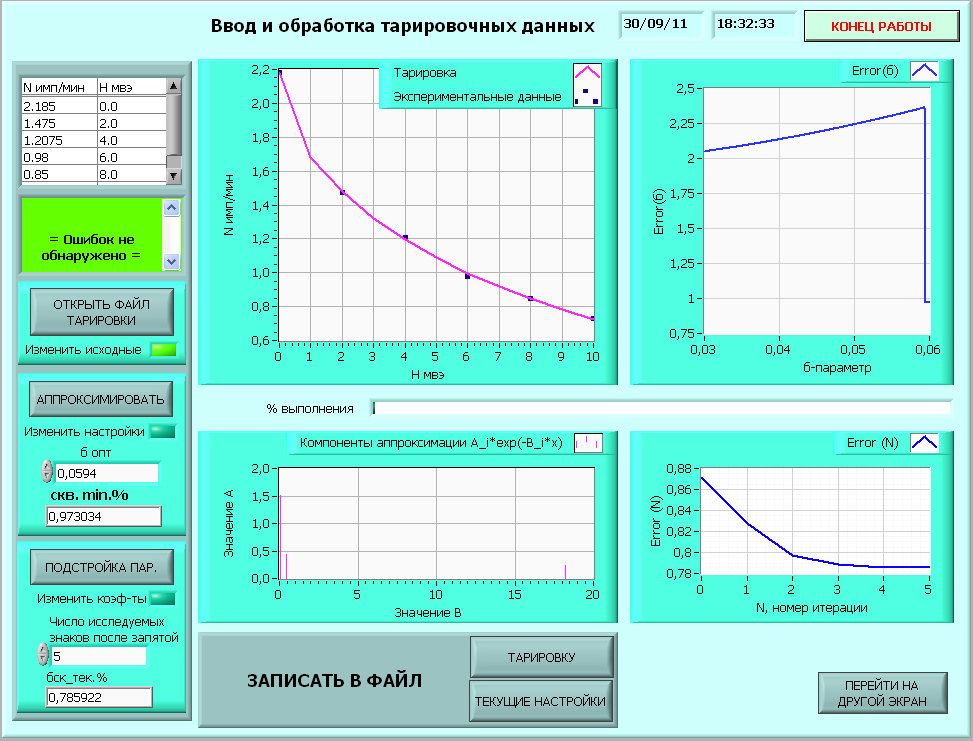
\includegraphics [scale=0.35] {operator}
  \caption{Интерфейс оператора по вводу и обработке тарировочных данных} 
  \label{img:operator} 

\end{figure}



Интерфейс оператора по обработке измерений (рис. \ref{img:operator_results}) предоставляет возможность ввода измеренных данных,
 проверку их корректности, а также, графическое и табличное отображение результатов обработки.
 Введенные данные измерений и результат обработки  можно сохранить в файле, а также,
 вывести на принтер (кнопка <<Распечатать>>) или скопировать для экспорта в другое приложение (кнопка <<Копировать в буфер обмена>>).



\begin{figure} [h]
  \center
  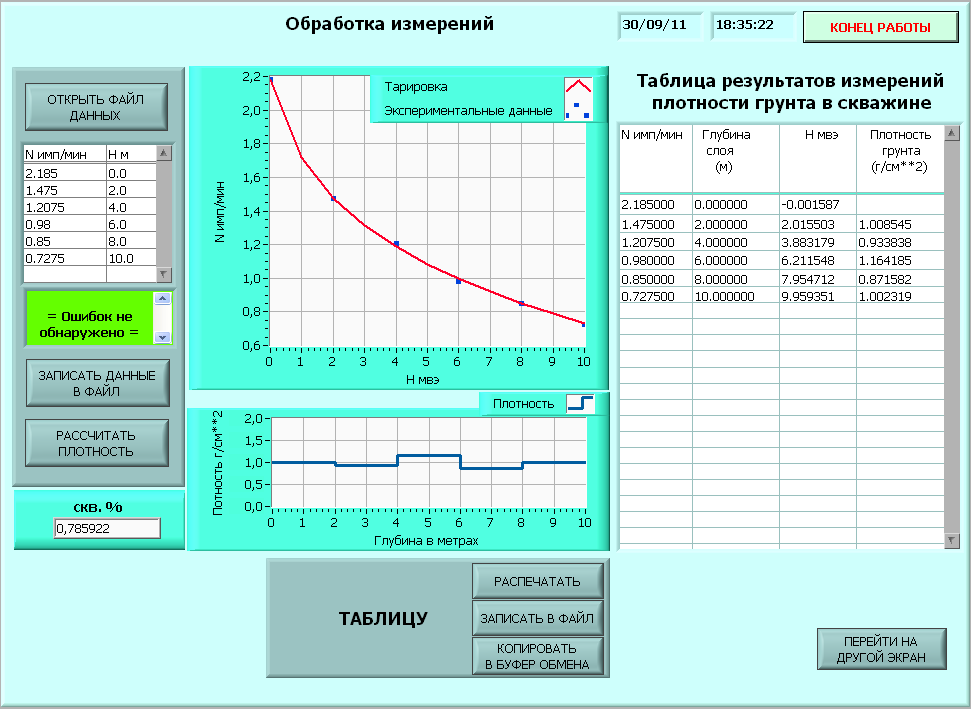
\includegraphics [scale=0.35] {operator_results}
  \caption{Интерфейс оператора по обработке измеренных данных} 
  \label{img:operator_results} 

\end{figure}


При анализе структуры созданного ПО выявлена возможность более тесной интеграции с пультом управления.
 Это позволило бы автоматизировать ввод данных, их оперативный обсчет и управление временем измерений.

\section{Метод определения неоднородностей в почве}

При проведении серии измерений, мюонный плотномер погружается в скважину и измеряет 
плотность потока мюонов на разных глубинах.
На результаты измерения влияют все предыдущие измеренные слои породы. Эта информация содержится в предыдущих 
измерениях и может быть использована для уменьшения погрешности текущего измерения или для пространственной локации неоднородностей.

В данной секции рассматривается метод определения неоднородностей в почве на основе серии измерений.

Были приняты следующие ограничения модели:

\begin{itemize}
\item Неоднородностью поверхности (напр. строительной площадки) можно пренебречь, и использовать бесконечную плоскость;
\item Плотность потока мюонов одинакова на всей поверхности площади;
\item Поток мюонов ослабляется в $\exp^{-r \rho}$ с увеличением пути, пройденного мюоном, где $r$ --- путь до детектора, а $\rho$ --- плотность породы
\item Принимается приближение точечного детектора \cite{kolcuzhkin} и бесконечного источника мюонов;
\item Задача имеет цилиндрическую симметрию.

\end{itemize}

\begin{figure} [h]
  \center
  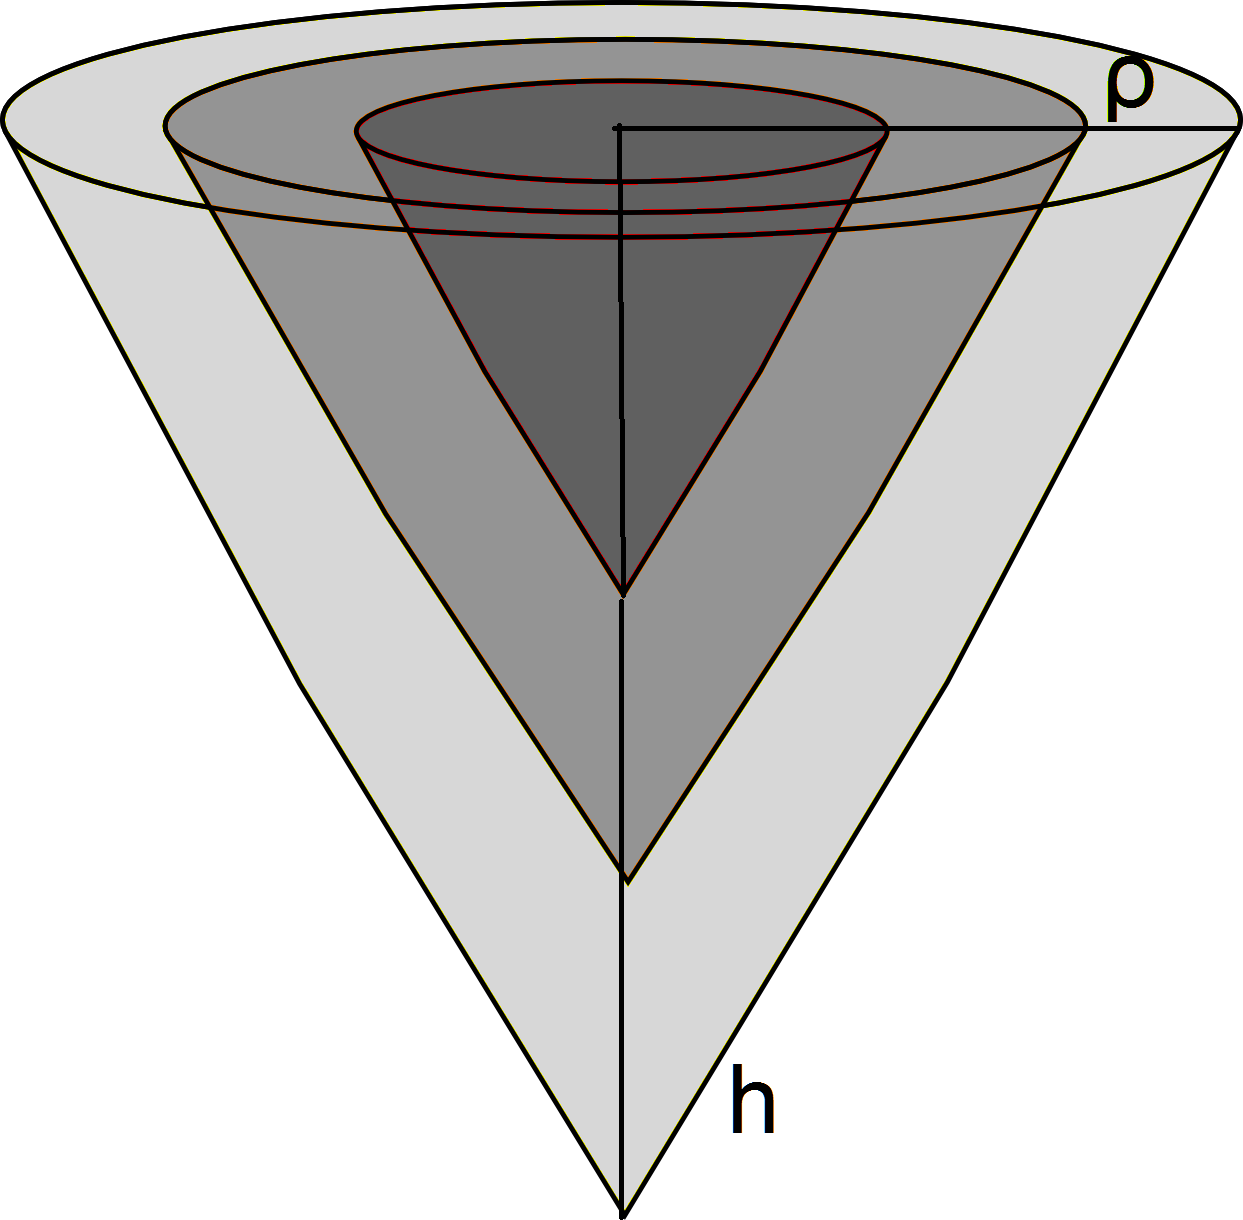
\includegraphics [scale=0.15] {cone_measure}
  \caption{Схематичное отображение измеряемых объемов} 
  \label{img:cone_measure} 

\end{figure}

При заданных ограничениях можно оценить эффективный угол, который получает 95\% измеренной величины потока мюонов

\begin{equation}
I(x) = 2 \pi \int_{0}^{r_{eff}} \exp^{\left( - \rho \sqrt{r^2 + h^2} \right) r^2 \, dr}
\end{equation}

Данный интеграл не имеет аналитического решения и $r_{eff}$ вместе с соответствующим ему $\theta_{eff}$ может быть 
оценен численно для характерных глубин. Для $h=0$ 
величина $\theta_{eff} = \pi / 2 - \pi / 12 $. 

Можно оценить численно объем измеренной породы в виде конуса с образующим углом
 $\theta_{eff}$: $V = \frac{1}{3} h^2 \cot{\theta_{eff}} $

Из величины интенсивности потока мюонов на заданной глубине, по тарировочной кривой можно получить плотность породы в 
заданном объеме. При серии измерений конусы оказываются вложенными друг в друга, при этом можно получить среднюю 
плотность в каждом из них. Вычитая массу и объем $i$-го конуса из $i+1$-го получаем: 

\begin{equation}
p_{i+1} = \frac{1}{3} \frac{\rho_{i+1} \left(h+1\right)^2 \cot{\theta_{i+1}} - \rho_{i} h^2 \cot{\theta_{i}} }{\left(h+1\right)^2 \cot{\theta_{i+1}} - h^2 \cot{\theta_{i}} }
\end{equation}

Корректированные значения $p_{i+1}$ показывают среднюю плотность между $i$ и $i+1$-ми конусами, что позволяет
выявлять неоднородности и локализовать их в меньшем объеме. Однако, данный метод не позволяет определить где именно 
находится неоднородность, а только указать цилиндрически-симметричный слой, в котором следует проводить поиски неоднородности.

Метод может быть расширен на случай с несколькими сериями пространственно разделенных измерений. При наличии 
частичного перекрытия, перекрывающийся объем учитывается по несколько раз. Применяя аналогичную итерационную схему 
можно рассчитать среднюю плотность породы между вложенными конусами, а также в местах перекрытия, что избавляет 
измерения от цилиндрической симметрии. При попадании неоднородности в места перекрытия, её положение явно определяется, 
в других случаях --- сокращается область поиска за счет области перекрытия.

\clearpage